\section{UserOption}
\label{sec:userOption}

\begin{figure}[h!] 
	\centering
	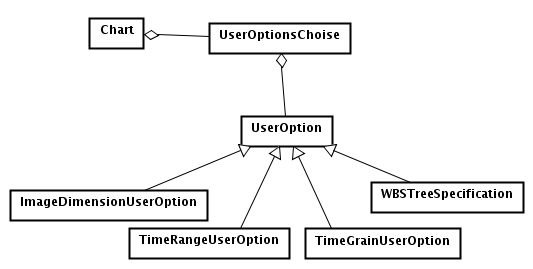
\includegraphics[width=0.7\textwidth]{../UserOptionDetail.png}
	\caption{UserOptions and choice}
	\label{fig:userOption} 
\end{figure}

Quando un generico client (potrebbe essere sia una persona fisica che un
oggetto astratto) della nostra implementazione della specifica vuole generare
un \emph{Chart} pu\`o guidare la generazione decidendo alcuni fattori che sono
di suo interesse. Questi fattori vengono modellati dal concetto di
\emph{UserOption}.

Ogni \emph{Chart} espone una lista di \emph{UserOption} per dare al client la
possibilit\`a di esprimere quali informazioni guidare. Questa lista varia da
\emph{Chart} a \emph{Chart}\footnote{creare un reference dove vengono mappate
questa relazione: potrebbe essere un appendici di questo documento??}.

Il concetto di lista di \emph{UserOption} \`e catturato in
\emph{UserOptionsChoice}.

Procediamo per passi: nelle prossime subsection osserviamo due aspetti che
trattarli insieme potrebbe non essere sufficiente per esporli in modo chiaro.

\subsection{\emph{UserOption}'s Instances}
Questa \`e stata una decisione non molto facile da prendere. Il problema \`e
questo: nella specifica abbiamo che per ogni \emph{Chart} il committente ha
dichiarato quali \emph{UserOption} mostrare. Queste per\`o non rappresentano un
concetto che vogliamo catturare nel nostro modello, ma allo stesso tempo sono
\emph{istanze} (un insieme discreto quindi) di elementi che fissa il
committente.

Per questo motivo decidiamo di codificare questo insieme discreto in questo
documento e la successiva enumerazione \`e da considerarsi parte integrante del
diagramma inserito come figura.

Rappresentiamo il concetto espresso sopra indicando due descrizioni con questa
struttura di codifica:
\begin{itemize}
  \item \emph{istanze}, dove inseriamo tutte le possibili \emph{UserOption} che
  non possono essere ancora raffinate
  \item \emph{specializzazioni} dove inseriamo tutte le possibili
  specializzazioni di \emph{UserOption} che possono essere ancora raffinate,
  ripetendo in modo ricorsivo questa struttura di codifica
\end{itemize}

Le successive descrizioni sono relative al concetto di \emph{UserOption}:
\begin{description}
  \item[istanze]\footnote{inserire qui la il mapping sui vari Chart?}
  \emph{WBSExplosionLevelUserOption, ActualTimeFrameOption, CompletitionBarOption, \\ PlannedDataOption, ActualDataOption,
  AlertMarkUserOption, ReplicateArrowUserOption, FindCriticalPathUserOption,
  WBSUserSpecificationUserLevel, \\WBSUserSpecificationUserLevel,
  ResourcesDetailsOption, TaskNameOption, CompleteDiagramUserOptions}
  \item[specializzazioni] \quad
  \begin{itemize}
    \item \emph{WBSTreeSpecification}
    \begin{description}
  \item[istanze] \emph{LevelSpecification, UserCustomSpecification}
  \item[specializzazioni] nessuna
\end{description}

\item \emph{TimeGrainUserOption}
    \begin{description}
  \item[istanze] \emph{WeaklyGrain, MonthlyGrain}
  \item[specializzazioni] nessuna
\end{description}

\item \emph{ImageDimensionUserOption}
    \begin{description}
  \item[istanze] \emph{CustomDim, FitInWindowDim, OptionalDim, DefaultDim}
  \item[specializzazioni] nessuna
\end{description}

\item \emph{TimeRangeUserOption}
    \begin{description}
  \item[istanze] \emph{CustomRange, WholeProjectRange, FromStartRange, ToEndRange}
  \item[specializzazioni] nessuna
\end{description}

  \end{itemize}
\end{description}

\subsection{\emph{UserOptionsChoice}}
Questo concetto \`e, secondo la nostra analisi, molto importante in quanto ci
permette di astrarre dal client che richiede una generazione.

Il motivo per cui abbiamo introdotto questo concetto \`e di poter lavorare lato
server usando \emph{UserOptionsChoice} per controllare quali informazioni il
client vuole guidare. In questo modo non siamo vincolati ad accedere ai dati
inviati per \emph{POST, GET} dalla form HTML, ma possiamo direttamente guardare
in \emph{UserOptionsChoice}. Queste ci permette di disaccopiare il processo di
generazione della maschera di input di una pagina HTML. 

Se vogliamo utilizzare il processo di generazione (che comunque \`e
server side) scrivendo un programma client (GUI o da riga di comando) che
costruisce una HTML request ad hoc (dovremo definire una grammatica e
attribuire la semantica ai contesti, questo \`e necessario, non ch\`e scrivere 
un parser), usando \emph{UserOptionsChoice} e il suo disaccoppiamento ci sar\`a
possibile farlo. 

Una volta ricevuta la response possiamo maneggiare la pagina
inviata come una response HTML valida e usarla per i nostri obiettivi (possiamo
rihiedere l'immagina generata, o il file PDF generato, salvandolo in
locale, oppure visualizzando lo stesso con un browser, ma possiamo anche
inserire in un db oppure farci dei test sopra\ldots).

Dovremo quindi costruire un oggetto che si incarica di costruire
\emph{UserOptionsChoice} in base al tipo di richiesta ricevuta (da una pagina
html come \`e il caso di PMango, oppure una richiesta da un client indipendente
scritto in un qualche linguaggio). Una volta costruito l'insieme delle
\emph{UserOption} \`e possibile iniziare la generazione. Questo sar\`a delegato
alla fase di progettazione.
